\begin{pastexam}[label={px:ntu-109-esoe-ds-08}]{臺大工科海洋所 109 學年度 第 8 題}
（追蹤）

\textbf{(10 \%)} What does the following splay tree look like after \textsf{remove(5)}?
\begin{center}
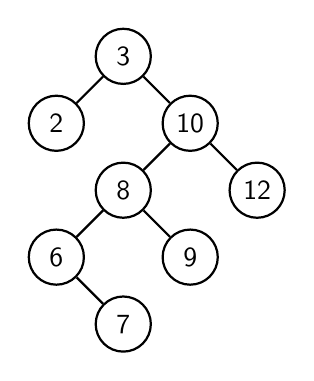
\begin{tikzpicture}[v/.style={circle,draw,thick,inner sep=1pt,minimum size=7mm,font=\sffamily},thick]
\node[v] (n3) at (0.85,0.00) {3};
\node[v] (n2) at (0.00,-0.85) {2};
\node[v] (n10) at (1.70,-0.85) {10};
\node[v] (n8) at (0.85,-1.70) {8};
\node[v] (n12) at (2.55,-1.70) {12};
\node[v] (n6) at (0.00,-2.55) {6};
\node[v] (n9) at (1.70,-2.55) {9};
\node[v] (n7) at (0.85,-3.40) {7};
\draw (n3) -- (n2);
\draw (n3) -- (n10);
\draw (n10) -- (n8);
\draw (n10) -- (n12);
\draw (n8) -- (n6);
\draw (n8) -- (n9);
\draw (n6) -- (n7);
\end{tikzpicture}
\end{center}
\end{pastexam}

\begin{pastsoln}
\textbf{注意：$5$ 不在樹裡。} 刪除用資結書第~10.6.2~節的做法（虛擬碼~10.11 \proc{Splay-Delete}）：先搜尋
$5$；找不到時，把搜尋路徑上最後經過的節點伸展到根（由下而上的伸展，虛擬碼~10.10），然後結束，
不刪任何節點。 「找不到也要伸展」是伸展樹平攤分析需要的，各家課本這一點大多相同（另一種常見的
刪除寫法是先照普通 BST 刪除、再伸展被刪節點的父節點，找不到時一樣是伸展最後經過的節點，結果相同）。

\textbf{搜尋 $5$}：$5 > 3$ 往右到 $10$；$5 < 10$ 往左到 $8$；$5 < 8$ 往左到 $6$；$5 < 6$ 要往左，但
$6$ 沒有左子節點。 最後經過的節點是 $6$，路徑是 $3 \to 10 \to 8 \to 6$。

\textbf{伸展 $6$}（資結書第~10.6.1~節）：
\begin{enumerate}
\item $6$ 是 $8$ 的左子節點，$8$ 是 $10$ 的左子節點，同一邊：\textbf{zig-zig}。 先對 $10$ 右旋，再對
$8$ 右旋。 結果以 $6$ 為根：$6$ 的右子節點是 $8$，$8$ 的左子節點是原本 $6$ 的右子樹 $7$，$8$ 的右子
節點是 $10$，$10$ 的左子節點是原本 $8$ 的右子樹 $9$，右子節點仍是 $12$。 這棵子樹接回 $3$ 的右邊。
\item $6$ 是根 $3$ 的右子節點：\textbf{zig}，對 $3$ 左旋。 $6$ 成為根，$3$ 成為 $6$ 的左子節點，$6$
原本的左子樹（空的）變成 $3$ 的右子樹。
\end{enumerate}

\begin{center}
\begin{tikzpicture}[v/.style={circle,draw,thick,inner sep=1pt,minimum size=7mm,font=\sffamily},thick,
    level distance=10mm, level 1/.style={sibling distance=18mm}, level 2/.style={sibling distance=12mm},
    level 3/.style={sibling distance=10mm}, every node/.style={v}]
\begin{scope}
\node {3}
  child {node {2}}
  child {node {6}
    child[missing]
    child {node {8}
      child {node {7}}
      child {node {10}
        child {node {9}}
        child {node {12}}}}};
\node[draw=none, font=\small] at (0.9,-5.0) {zig-zig 之後};
\end{scope}
\begin{scope}[xshift=6.5cm]
\node {6}
  child {node {3}
    child {node {2}}
    child[missing]}
  child {node {8}
    child {node {7}}
    child {node {10}
      child {node {9}}
      child {node {12}}}};
\node[draw=none, font=\small] at (0,-4.0) {zig 之後（答案）};
\end{scope}
\end{tikzpicture}
\end{center}

答案：根是 $6$；$6$ 的左子節點 $3$（$3$ 的左子節點 $2$）；$6$ 的右子節點 $8$，$8$ 的子節點是 $7$ 和
$10$，$10$ 的子節點是 $9$ 和 $12$。 中序 $2, 3, 6, 7, 8, 9, 10, 12$，和原本一樣，仍是 BST。

如果題目的意思是樹裡有 $5$（例如原圖漏畫），做法是：把 $5$ 伸展到根、拿掉它，在左子樹找最大的節點
伸展到左子樹的根，再把右子樹接到它的右邊。 照原圖，$5$ 確實不在樹裡，所以答案是上面伸展 $6$ 的結果。
\end{pastsoln}
